
\documentclass{IOS-Book-Article}

\usepackage{mathptmx}
\usepackage{soul}\setuldepth{article}
\usepackage{graphicx}
\graphicspath{ {./figures/} }
%\usepackage{times}
%\normalfont
%\usepackage[T1]{fontenc}
%\usepackage[mtplusscr,mtbold]{mathtime}
%
\def\hb{\hbox to 11.5 cm{}}

\begin{document}

\pagestyle{headings}
\def\thepage{}
\begin{frontmatter}              % The preamble begins here.


%\pretitle{Pretitle}
\title{First Steps towards a Risk of Bias Corpus of Randomized Controlled Trials}

\markboth{}{April 2022\hb}
%\subtitle{Subtitle}

\author[A,B]{\fnms{Anjani} \snm{Dhrangadhariya}\orcid{0000-0003-1691-1338}%
\thanks{Corresponding Author: Anjani Dhrangadhariya, Informatics Institute, HES-SO Valais-Wallis, Technopole 3,
3960 Sierre, Switzerland; E-mail:
anjani.dhrangadhariya@hevs.ch.}},
\author[C,D]{\fnms{Roger} \snm{Hilfiker}}
,
\author[C,D]{\fnms{Martin} \snm{Sattlemayer}}
,
\author[C,D]{\fnms{Katia} \snm{Giacomino}}
,
\author[C,D]{\fnms{Rahel} \snm{Caliesch}}
,
\author[C,D]{\fnms{Simone} \snm{Elsig}}
,
\author[E,F]{\fnms{Nona} \snm{Naderi}}
and
\author[A,B]{\fnms{Henning} \snm{M\"uller}}

\runningauthor{A. Dhrangadhariya et al.}
\address[A]{Informatics Institute, HES-SO Valais-Wallis, Sierre, Switzerland}
\address[B]{University of Geneva (UNIGE), Geneva, Switzerland}
\address[C]{School of Health Sciences, HES-SO Valais-Wallis, Leukerbad, Switzerland.}
\address[D]{Department of Physiotherapy, HES-SO Valais-Wallis, Leukerbad, Switzerland.}
\address[E]{Geneva School of Business Administration, HES-SO Geneva, Switzerland.}
\address[F]{SIB Swiss Institute of Bioinformatics (SIB), Geneva, Switzerland}

\begin{abstract}
Risk of bias (RoB) assessment of randomized clinical trials (RCTs) is vital to conducting systematic reviews. 
Manual RoB assessment for hundreds of RCTs is a cognitively demanding, lengthy process and is prone to subjective judgment. 
Supervised machine learning (ML) can help to accelerate this process but requires a hand-labelled corpus.
There are currently no RoB annotation guidelines for randomized clinical trials or any annotated corpora.
In this pilot project, we test the practicality of directly using the revised Cochrane RoB 2.0 tool for developing an RoB annotated corpus with a novel multi-level annotation scheme.
We report inter-annotator agreement among four experienced annotators, which ranges between 0\% for some bias classes and 76\% for others.
Finally, we discuss the shortcomings of this direct translation of annotation guidelines and scheme and suggest approaches to improve them to obtain an RoB annotated corpus suitable for ML.
\end{abstract}

\begin{keyword}
risk of bias\sep annotation\sep
systematic reviews\sep corpus\sep automation
\end{keyword}
\end{frontmatter}
\markboth{April 2022\hb}{April 2022\hb}
%\thispagestyle{empty}
%\pagestyle{empty}
%
%
%
\section{Introduction}
\label{sec:intro}
%
Systematic reviews (SRs) synthesized from randomized controlled trials (RCTs) are the highest quality of evidence in the evidence hierarchy.
In theory, an RCT accurately measures the treatment effect on patient outcomes but can be biased in practice due to flawed study design, execution, analysis or outcome reporting.~\cite{hariton2018randomised}
Biases in RCTs cannot be measured, but the risk of bias (RoB) can be assessed.
The researchers conducting SRs must rigorously look for possible biases before incorporating them into SRs.
Published RCTs are exponentially increasing~\footnote{\url{https://pubmed.ncbi.nlm.nih.gov/?term=randomized\%20controlled\%20trial&filter=pubt.randomizedcontrolledtrial}} over time, so manual assessment for every study becomes a protracted process.
Machine learning (ML) can help accelerate this process by directly pointing the reviewers to the parts of the text relevant to identifying RoB, leading to quickly judging the trial quality.
Both Marshall \textit{et al.} and Millard \textit{et al.} attempted automated RoB assessment, albeit using proprietary, pay-walled data.~\cite{marshall2015automating,millard2016machine}
Recently, Wang \textit{et al.} released a hand-labelled RoB corpus for animal studies using a preclinical RoB assessment tool.~\cite{wang2022risk}
RoB assessment is a knowledge-heavy task where even highly trained experts are prone to subjective judgments.
The primary requirement to develop such a corpus entails creating a clear-cut annotation scheme and guidelines.
As neither exists, this work focuses on two primary concerns.
1) To test whether the widely used revised Cochrane's RoB 2.0 tool for RCTs (RoB 2.0) could be used as RoB annotation guidelines to develop a corpus that could be used for training supervised ML models.~\cite{lansbury2020co}
2) To develop and test an RoB annotation scheme that closely mimics the RoB 2.0.~\cite{sterne2019rob}
%
%
%
\section{Methods}
\label{sec:methods}
%
\subsection{Formulating Annotation Scheme}
%
%We formulate the annotation scheme as a function of the RoB 2.0 tool.
RoB 2.0 tool divides biases into five risk domains which further decompose into several signalling questions, each corresponding to different parts of the trial design.
Each signalling question prompts the reviewer to look for a piece(s) of factual evidence in the RCT to respond with one of the five response options: ``Yes'', ``Probably yes'', ``No'', ``Probably no'', or ``No information''.
E.g. to respond to the signalling question ``Was the allocation sequence random?'', the reviewers need to identify whether a proper methodology was used for random participant allocation and only if a proper methodology is identified the reviewer responds to this question as ``Yes'' and otherwise ``No''.

We formulated an annotation scheme where each signalling question is an entity.
Each entity has five entity labels corresponding to the five response options to that question.
Entities represent the factual evidence from the RCTs, and the entity labels incorporate the reviewer's risk judgment.
The cumulative risk judgment (``Low-risk'', ``High-risk'' or ``Some-concerns'') from each risk domain was estimated using decision flowcharts in RoB 2.0, combining the responses from all the signalling questions.
To account for this, we had an additional document-level annotation for each risk domain whereby a reviewer chose either of the three risk judgments.
A visual representation of our annotation scheme is illustrated in Figure~\ref{fig:ann_scheme}.
%
\begin{figure}[!htbp]
    \centering
    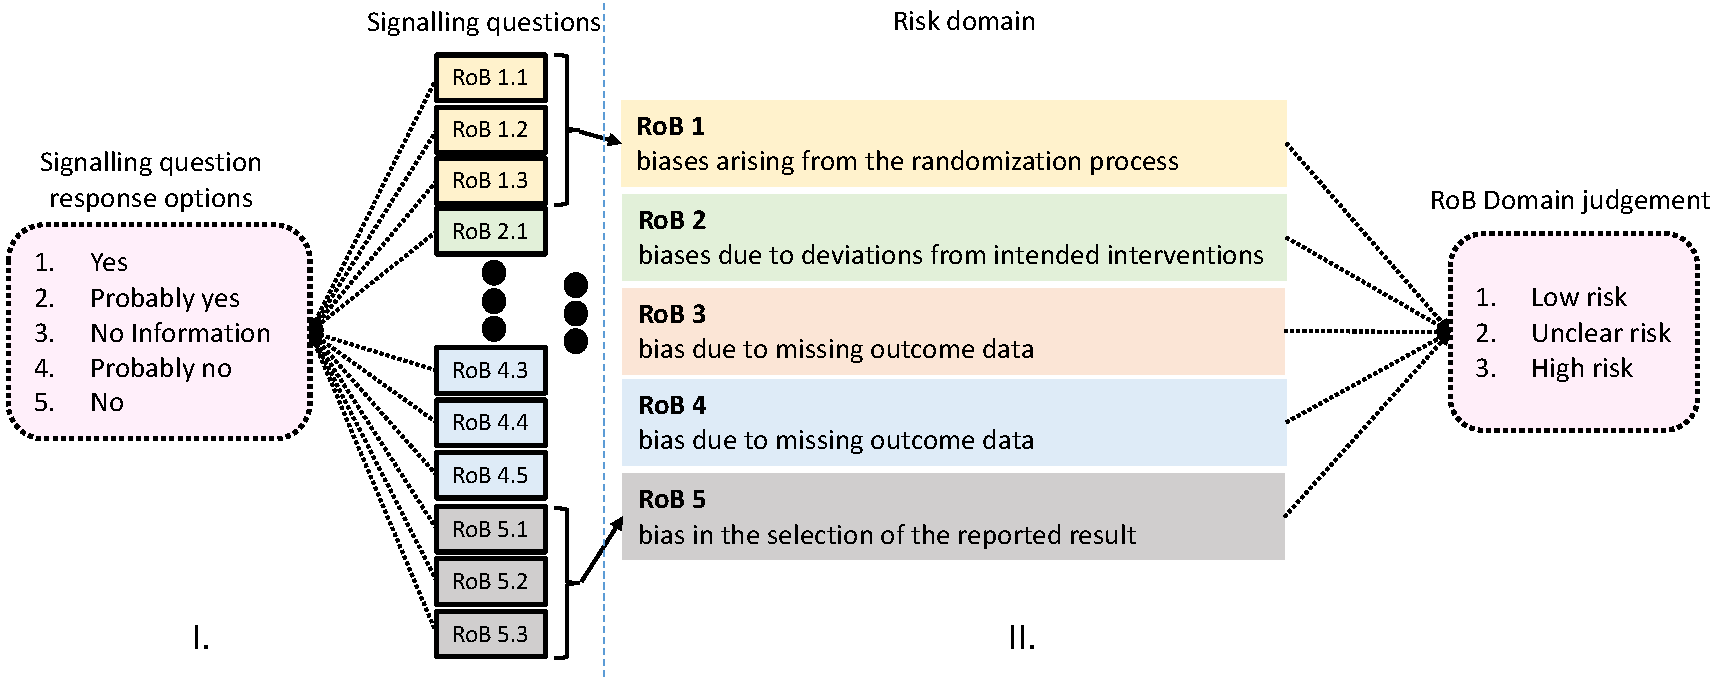
\includegraphics[width=0.80\textwidth]{Figures/annotation_scheme.pdf}
    \caption{Annotation scheme. I. Signalling question: each signalling question (RoB 1.1, 1.2, ...) is an entity that could take either of five response options (entity labels). II. Risk domain: each risk domain (RoB 1-5) is a document label that could take either of three risk classes based on assessment of all RoB signalling questions.}
    \label{fig:ann_scheme}
\end{figure}
%
%
%
\subsection{Preliminary Annotation guidelines}
\label{subsec:annot_guide}
%
Full-text RCTs were annotated using the RoB assessment instructions from the RoB 2.0.~\footnote{\url{https://drive.google.com/file/d/19R9savfPdCHC8XLz2iiMvL_71lPJERWK/view}}
A.D. developed the generic annotation guidelines with four physiotherapists experienced in bias assessment to ensure consistency.
Complete sentence(s) or phrase(s) were annotated depending upon the text parts relevant to answering a signalling question.
All the text information pertinent to answering a question was marked, even if the information was found in different parts of the full text.
Table or figure captions relevant to answering were marked.
If the information was not found in the captions, it was marked within the table contents.
If a reference to the table or figure led to answering the question, it was annotated.
If all three were relevant then all were annotated.
%
\subsection{Pilot annotation}
\label{subsec:annotation}
%
The four physiotherapists (R.H., M.S., K.G., R.C.), who consented to annotating, did the pilot annotation on a corpus of ten RCTs sampled in the following manner.
An Entrez~\footnote{The Entrez Global Query Cross-Database Search System is a federated search engine or web portal that allows users to search PubMed database} search using the search query ``{\fontfamily{qcr}\selectfont (randomized[title] or randomized[title]) and (rehabilitation or (physical therapy))}'' was performed ten times to retrieve studies from one-year time-spans each between 2000 - 2019.
Each query was restricted to retrieve 1000 documents, of which ten were randomly chosen for each time span.
Of the ten sampled studies, R.H. took the first possible study with a freely available PDF.
R.H. and M.S. are professors and associate professors, respectively, and K.G. and R.C. are doctoral researchers with experience conducting RoB ratings in several SRs.


Tagtog\footnote{\url{https://www.tagtog.com/}}, a commercial tool, was used for annotating the full-text PDFs (Portable Document Format).
The task for the annotator was to annotate text relevant to answering each signalling question entity, choose a judgment response option, and finally select the risk domain judgment for the five risk domains.

We report token-level pairwise F1 measure as an inter-annotator agreement (IAA) for the entity $IAA_{sq}$ and entity label $IAA_{response}$
annotations.~\cite{brandsen2020creating,deleger2012building}
$IAA_{sq}$ and $IAA_{response}$ measure reliability of the RoB 2.0 guidelines for selecting the same parts of the text to answering signalling questions.
Cohen's Kappa was chosen for the document-level $IAA_{rd}$ agreements.~\cite{mchugh2012interrater}
%
%
%
\section{Results}
\label{sec:results}
%
The pilot annotation resulted in 902 RoB entity labels corresponding to the signalling question categories and 220 risk domain class labels at the document level.
The Table \ref{tab:iaa_sq_res} reports pairwise $IAA_{sq}$ (left side) between the six annotator pairs (P1-P6) and the $IAA_{response}$ (right side) averaged over all the annotator pairs at the signalling question response option level.
Individual pairwise agreements $IAA_{sq}$ range between 0\% (poor) and 75\% (substantial), with most values falling under the poor category and very few under the substantial agreement.
``-'' denotes either of the pair did not annotate for the entity. 
Signalling questions RoB 1.1, 1.2, 1.3, 2.6, and 3.1 fared well in terms of the average pairwise agreement between all pairs, but none of these categories had a substantial agreement.
Signalling questions 2.3, 2.4, 2.5, 2.7, 3.4, 4.4, 4.5, and entire domain 5 fared extremely poorly or with no agreement or annotation.
The $IAA_{response}$ scores are considerably lower (to zero) than agreement at the signalling question level ($IAA_{sq}$), hinting that annotators assign different response options for the text relevant to answering a signalling question. 
Most annotators had zero agreement or did not annotate any text relevant to answering the signalling questions for this domain.


\begin{table}[!ht]
    \centering
    \begin{tabular}{|l||l|l|l|l|l|l|l||l|l|l|l|l|}
    \hline
        SQ & P1 & P2 & P3 & P4 & P5 & P6 & Avg & Y & PY & NI & PN & N \\ \hline \hline
        1.1 & 23.1 & 24.5 & 52.2 & 57.0 & 48.0 & 21.5 & 37.7 & 21.8 & 7.1 & 0.0 & - & - \\ 
        1.2 & 66.1 & 50.3 & 72.8 & 50.7 & 46.0 & 50.5 & 56.1 & 4.9 & 11.5 & 10.2 & 0.0 & - \\ 
        1.3 & 69.5 & 20.5 & 16.1 & 31.6 & 59.9 & 53.5 & 41.8 & - & - & 41.8 & 11.4 & 9.9 \\ \hline
        2.1 & 1.0 & 1.4 & 0.0 & 9.1 & 19.1 & 0.0 & 5.1 & 8.2 & 0.0 & - & 3.0 & 0.0 \\ 
        2.2 & 18.3 & 7.3 & 11.1 & 0.0 & 23.0 & 7.4 & 11.2 & 3.6 & 0.0 & 0.0 & 0.0 & 0.0 \\ 
        2.3 & 20.6 & 5.5 & 13.4 & 0.0 & 0.0 & 0.0 & 6.6 & - & 0.0 & - & 1.0 & 0.0 \\ 
        2.4 & 0 & - & - & 0 & 0 & - & 0 & - & 0 & - & 0 & - \\ 
        2.5 & 0 & 0 & 0 & 0 & 0 & - & 0 & 0 & 0 & - & 0 & - \\ 
        2.6 & 75.3 & 68.9 & 19.3 & 63.9 & 12.9 & 19.6 & 43.3 & 39.4 & 0.0 & 0.0 & 0.0 & 3.6 \\ 
        2.7 & 0.0 & 6.6 & 0.0 & 0.0 & 0.0 & 0.0 & 1.1 & 0.0 & 0.0 & - & 0.0 & 0.0 \\ \hline
        3.1 & 45.8 & 23.6 & 32.2 & 43.4 & 22.9 & 14.8 & 30.4 & 47.6 & 0.6 & - & 1.3 & 3.3 \\ 
        3.2 & 1.4 & 0.0 & 0.0 & 3.3 & 7.4 & 0.9 & 2.2 & 0.0 & 0.0 & - & 0.0 & 0.0 \\ 
        3.3 & 0.0 & 0.0 & 0.0 & 16.4 & 0.0 & 0.0 & 2.8 & - & 0.0 & 31.4 & 0.0 & 0.0 \\ 
        3.4 & - & 0 & - & 0 & 0 & 0 & 0 & 0 & 0 & 0 & 0 & 0 \\ \hline
        4.1 & 4.0 & 6.6 & 14.2 & 25.6 & 22.3 & 6.3 & 13.2 & - & - & - & 0.8 & 12.0 \\ 
        4.2 & 1.8 & 0.0 & 0.4 & 0.0 & 40.1 & 0.0 & 7.1 & - & - & - & 0.3 & 0.0 \\
        4.3 & 7.6 & 13.9 & 5.0 & 10.5 & 39.5 & 8.4 & 14.2 & 0.0 & 0.0 & 0.0 & 13.1 & 20.5 \\ 
        4.4 & 0 & 0 & 0 & 0 & 0 & 0 & 0 & 0 & 0 & - & 0 & 0 \\ 
        4.5 & 0 & 0 & 0 & 0 & 0 & 0 & 0 & 0 & 0 & - & 0 & - \\ \hline
        5.1 & 0.0 & 0.0 & 0.0 & 0.0 & 0.0 & 4.2 & 0.7 & 0.0 & 0.0 & 0.0 & 0.0 & 0.0 \\ 
        5.2 & 23.9 & 0.0 & 0.0 & 0.0 & 0.0 & 2.4 & 4.4 & - & 0.0 & 0.0 & 0.0 & 0.0 \\ 
        5.3 & 0.2 & 0.0 & 0.0 & 0.4 & 8.1 & 42.0 & 8.4 & - & 0.0 & 0.6 & 0.0 & 0.0 \\ \hline
    \end{tabular}
    \caption{\label{tab:iaa_sq_res} Left Side: The table lists down $IAA_{sq}$ between the pair of annotators for the risk of bias signalling questions at the text evidence level. Note: A dash (-) shows that one of the annotators did not annotate any text for a particular signalling question. Right side: The table lists down the inter-annotator agreement $IAA_{sq}$ averaged over the six annotator pairs for the risk of bias signalling questions at the ``response'' option level. Note: SQ = Signalling Question, Y = Yes, PY = Probably Yes, NI = No Information, N = No and PN = Probably No. Note: SQ = Signalling Question, Avg. = Average}
\end{table}

%
%
%
\section{Discussion}

\section{Conclusion}
\label{sec:conclusion}
%
We conclude that RoB 2.0 tool cannot be directly used as RoB corpus annotation guidelines.
The annotation scheme directly adapted from RoB 2.0 document also needs improvement, as detailed in the discussion.
Currently, we are using the insights from this pilot project to develop crisp annotation guidelines to obtain consistent annotations.
The annotated dataset is available on Zenodo.
%
%
%
%%%%% References %%%%%
\bibliographystyle{spiebib} 
%
%
\bibliography{bibliography}
%
\end{document}
